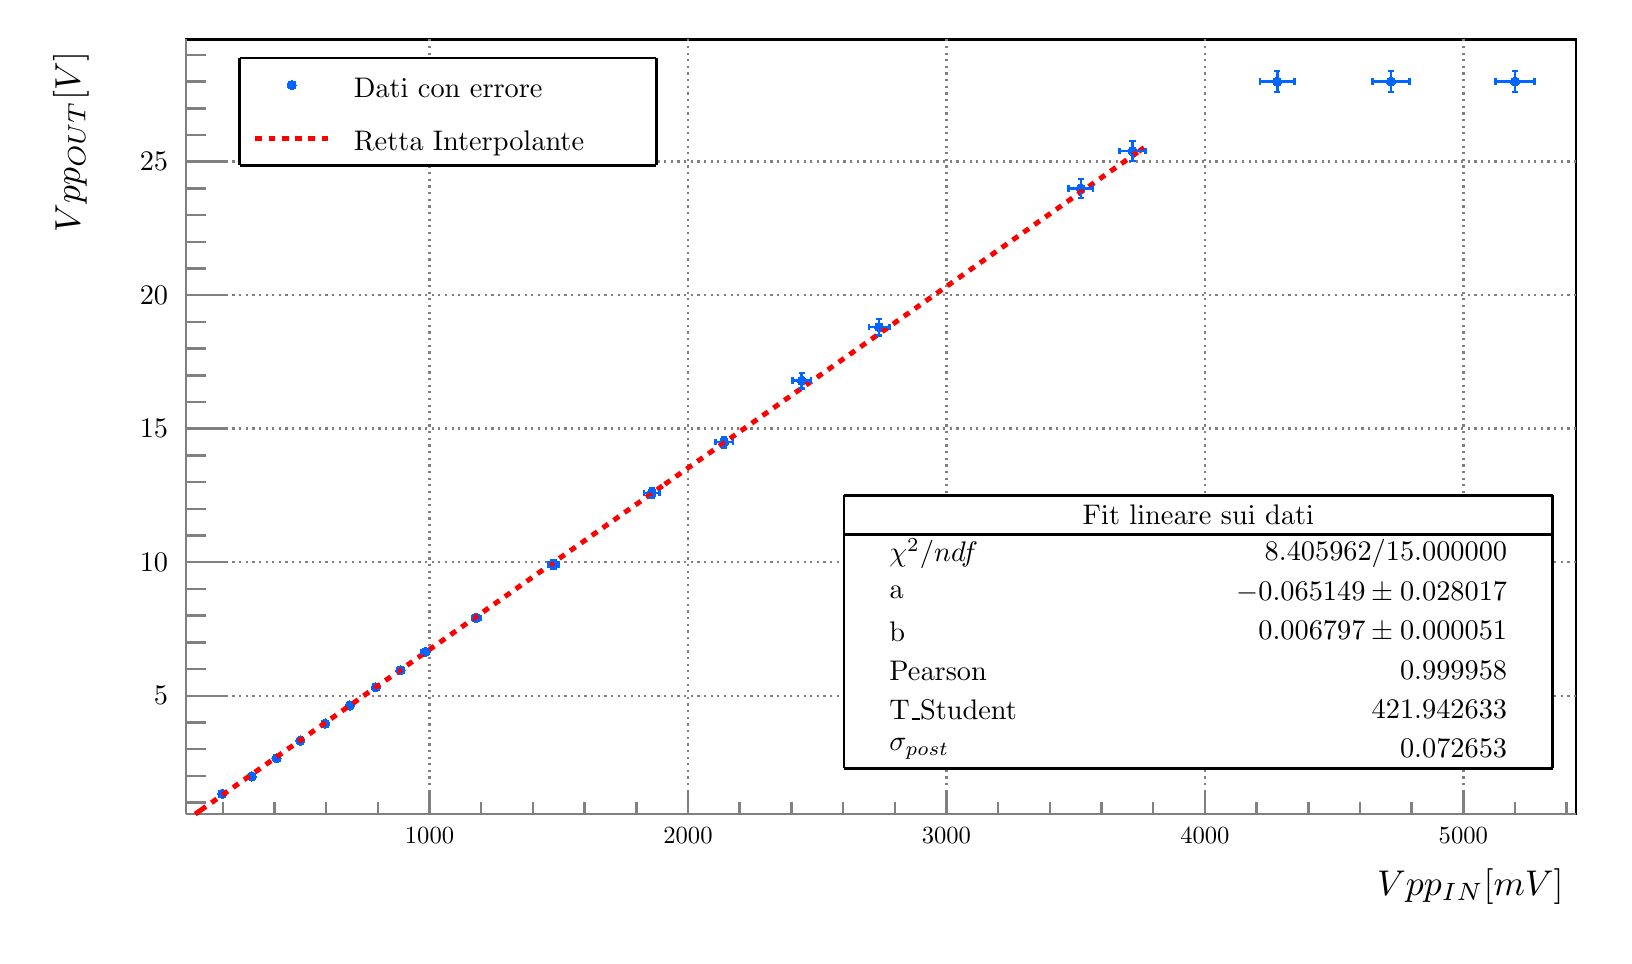
\begin{tikzpicture}
\pgfdeclareplotmark{cross} {
\pgfpathmoveto{\pgfpoint{-0.3\pgfplotmarksize}{\pgfplotmarksize}}
\pgfpathlineto{\pgfpoint{+0.3\pgfplotmarksize}{\pgfplotmarksize}}
\pgfpathlineto{\pgfpoint{+0.3\pgfplotmarksize}{0.3\pgfplotmarksize}}
\pgfpathlineto{\pgfpoint{+1\pgfplotmarksize}{0.3\pgfplotmarksize}}
\pgfpathlineto{\pgfpoint{+1\pgfplotmarksize}{-0.3\pgfplotmarksize}}
\pgfpathlineto{\pgfpoint{+0.3\pgfplotmarksize}{-0.3\pgfplotmarksize}}
\pgfpathlineto{\pgfpoint{+0.3\pgfplotmarksize}{-1.\pgfplotmarksize}}
\pgfpathlineto{\pgfpoint{-0.3\pgfplotmarksize}{-1.\pgfplotmarksize}}
\pgfpathlineto{\pgfpoint{-0.3\pgfplotmarksize}{-0.3\pgfplotmarksize}}
\pgfpathlineto{\pgfpoint{-1.\pgfplotmarksize}{-0.3\pgfplotmarksize}}
\pgfpathlineto{\pgfpoint{-1.\pgfplotmarksize}{0.3\pgfplotmarksize}}
\pgfpathlineto{\pgfpoint{-0.3\pgfplotmarksize}{0.3\pgfplotmarksize}}
\pgfpathclose
\pgfusepathqstroke
}
\pgfdeclareplotmark{cross*} {
\pgfpathmoveto{\pgfpoint{-0.3\pgfplotmarksize}{\pgfplotmarksize}}
\pgfpathlineto{\pgfpoint{+0.3\pgfplotmarksize}{\pgfplotmarksize}}
\pgfpathlineto{\pgfpoint{+0.3\pgfplotmarksize}{0.3\pgfplotmarksize}}
\pgfpathlineto{\pgfpoint{+1\pgfplotmarksize}{0.3\pgfplotmarksize}}
\pgfpathlineto{\pgfpoint{+1\pgfplotmarksize}{-0.3\pgfplotmarksize}}
\pgfpathlineto{\pgfpoint{+0.3\pgfplotmarksize}{-0.3\pgfplotmarksize}}
\pgfpathlineto{\pgfpoint{+0.3\pgfplotmarksize}{-1.\pgfplotmarksize}}
\pgfpathlineto{\pgfpoint{-0.3\pgfplotmarksize}{-1.\pgfplotmarksize}}
\pgfpathlineto{\pgfpoint{-0.3\pgfplotmarksize}{-0.3\pgfplotmarksize}}
\pgfpathlineto{\pgfpoint{-1.\pgfplotmarksize}{-0.3\pgfplotmarksize}}
\pgfpathlineto{\pgfpoint{-1.\pgfplotmarksize}{0.3\pgfplotmarksize}}
\pgfpathlineto{\pgfpoint{-0.3\pgfplotmarksize}{0.3\pgfplotmarksize}}
\pgfpathclose
\pgfusepathqfillstroke
}
\pgfdeclareplotmark{newstar} {
\pgfpathmoveto{\pgfqpoint{0pt}{\pgfplotmarksize}}
\pgfpathlineto{\pgfqpointpolar{44}{0.5\pgfplotmarksize}}
\pgfpathlineto{\pgfqpointpolar{18}{\pgfplotmarksize}}
\pgfpathlineto{\pgfqpointpolar{-20}{0.5\pgfplotmarksize}}
\pgfpathlineto{\pgfqpointpolar{-54}{\pgfplotmarksize}}
\pgfpathlineto{\pgfqpointpolar{-90}{0.5\pgfplotmarksize}}
\pgfpathlineto{\pgfqpointpolar{234}{\pgfplotmarksize}}
\pgfpathlineto{\pgfqpointpolar{198}{0.5\pgfplotmarksize}}
\pgfpathlineto{\pgfqpointpolar{162}{\pgfplotmarksize}}
\pgfpathlineto{\pgfqpointpolar{134}{0.5\pgfplotmarksize}}
\pgfpathclose
\pgfusepathqstroke
}
\pgfdeclareplotmark{newstar*} {
\pgfpathmoveto{\pgfqpoint{0pt}{\pgfplotmarksize}}
\pgfpathlineto{\pgfqpointpolar{44}{0.5\pgfplotmarksize}}
\pgfpathlineto{\pgfqpointpolar{18}{\pgfplotmarksize}}
\pgfpathlineto{\pgfqpointpolar{-20}{0.5\pgfplotmarksize}}
\pgfpathlineto{\pgfqpointpolar{-54}{\pgfplotmarksize}}
\pgfpathlineto{\pgfqpointpolar{-90}{0.5\pgfplotmarksize}}
\pgfpathlineto{\pgfqpointpolar{234}{\pgfplotmarksize}}
\pgfpathlineto{\pgfqpointpolar{198}{0.5\pgfplotmarksize}}
\pgfpathlineto{\pgfqpointpolar{162}{\pgfplotmarksize}}
\pgfpathlineto{\pgfqpointpolar{134}{0.5\pgfplotmarksize}}
\pgfpathclose
\pgfusepathqfillstroke
}
\definecolor{c}{rgb}{1,1,1};
\draw [color=c, fill=c] (0,0) rectangle (20,11.523);
\draw [color=c, fill=c] (2.00401,1.54309) rectangle (19.6593,11.3828);
\definecolor{c}{rgb}{0,0,0};
\draw [c,line width=0.9] (2.00401,1.54309) -- (2.00401,11.3828) -- (19.6593,11.3828) -- (19.6593,1.54309) -- (2.00401,1.54309);
\definecolor{c}{rgb}{1,1,1};
\draw [color=c, fill=c] (2.00401,1.54309) rectangle (19.6593,11.3828);
\definecolor{c}{rgb}{0,0,0};
\draw [c,line width=0.9] (2.00401,1.54309) -- (2.00401,11.3828) -- (19.6593,11.3828) -- (19.6593,1.54309) -- (2.00401,1.54309);
\definecolor{c}{rgb}{0.5,0.5,0.5};
\draw [c,line width=0.9] (2.00401,1.54309) -- (19.6593,1.54309);
\draw [c,dash pattern=on 0.80pt off 1.60pt ,line width=0.9] (5.09651,11.3828) -- (5.09651,1.54309);
\draw [c,dash pattern=on 0.80pt off 1.60pt ,line width=0.9] (8.37886,11.3828) -- (8.37886,1.54309);
\draw [c,dash pattern=on 0.80pt off 1.60pt ,line width=0.9] (11.6612,11.3828) -- (11.6612,1.54309);
\draw [c,dash pattern=on 0.80pt off 1.60pt ,line width=0.9] (14.9436,11.3828) -- (14.9436,1.54309);
\draw [c,dash pattern=on 0.80pt off 1.60pt ,line width=0.9] (18.2259,11.3828) -- (18.2259,1.54309);
\draw [c,dash pattern=on 0.80pt off 1.60pt ,line width=0.9] (5.09651,11.3828) -- (5.09651,1.54309);
\draw [c,dash pattern=on 0.80pt off 1.60pt ,line width=0.9] (18.2259,11.3828) -- (18.2259,1.54309);
\draw [c,line width=0.9] (2.00401,1.54309) -- (2.00401,11.3828);
\draw [c,dash pattern=on 0.80pt off 1.60pt ,line width=0.9] (19.6593,3.04514) -- (2.00401,3.04514);
\draw [c,dash pattern=on 0.80pt off 1.60pt ,line width=0.9] (19.6593,4.74088) -- (2.00401,4.74088);
\draw [c,dash pattern=on 0.80pt off 1.60pt ,line width=0.9] (19.6593,6.43662) -- (2.00401,6.43662);
\draw [c,dash pattern=on 0.80pt off 1.60pt ,line width=0.9] (19.6593,8.13236) -- (2.00401,8.13236);
\draw [c,dash pattern=on 0.80pt off 1.60pt ,line width=0.9] (19.6593,9.8281) -- (2.00401,9.8281);
\draw [c,dash pattern=on 0.80pt off 1.60pt ,line width=0.9] (19.6593,3.04514) -- (2.00401,3.04514);
\draw [c,dash pattern=on 0.80pt off 1.60pt ,line width=0.9] (19.6593,9.8281) -- (2.00401,9.8281);
\draw [c,line width=0.9] (2.00401,1.54309) -- (19.6593,1.54309);
\draw [c,line width=0.9] (5.09651,1.84825) -- (5.09651,1.54309);
\draw [c,line width=0.9] (5.75298,1.69567) -- (5.75298,1.54309);
\draw [c,line width=0.9] (6.40945,1.69567) -- (6.40945,1.54309);
\draw [c,line width=0.9] (7.06592,1.69567) -- (7.06592,1.54309);
\draw [c,line width=0.9] (7.72239,1.69567) -- (7.72239,1.54309);
\draw [c,line width=0.9] (8.37886,1.84825) -- (8.37886,1.54309);
\draw [c,line width=0.9] (9.03533,1.69567) -- (9.03533,1.54309);
\draw [c,line width=0.9] (9.6918,1.69567) -- (9.6918,1.54309);
\draw [c,line width=0.9] (10.3483,1.69567) -- (10.3483,1.54309);
\draw [c,line width=0.9] (11.0047,1.69567) -- (11.0047,1.54309);
\draw [c,line width=0.9] (11.6612,1.84825) -- (11.6612,1.54309);
\draw [c,line width=0.9] (12.3177,1.69567) -- (12.3177,1.54309);
\draw [c,line width=0.9] (12.9741,1.69567) -- (12.9741,1.54309);
\draw [c,line width=0.9] (13.6306,1.69567) -- (13.6306,1.54309);
\draw [c,line width=0.9] (14.2871,1.69567) -- (14.2871,1.54309);
\draw [c,line width=0.9] (14.9436,1.84825) -- (14.9436,1.54309);
\draw [c,line width=0.9] (15.6,1.69567) -- (15.6,1.54309);
\draw [c,line width=0.9] (16.2565,1.69567) -- (16.2565,1.54309);
\draw [c,line width=0.9] (16.913,1.69567) -- (16.913,1.54309);
\draw [c,line width=0.9] (17.5694,1.69567) -- (17.5694,1.54309);
\draw [c,line width=0.9] (18.2259,1.84825) -- (18.2259,1.54309);
\draw [c,line width=0.9] (5.09651,1.84825) -- (5.09651,1.54309);
\draw [c,line width=0.9] (4.44004,1.69567) -- (4.44004,1.54309);
\draw [c,line width=0.9] (3.78357,1.69567) -- (3.78357,1.54309);
\draw [c,line width=0.9] (3.1271,1.69567) -- (3.1271,1.54309);
\draw [c,line width=0.9] (2.47064,1.69567) -- (2.47064,1.54309);
\draw [c,line width=0.9] (18.2259,1.84825) -- (18.2259,1.54309);
\draw [c,line width=0.9] (18.8824,1.69567) -- (18.8824,1.54309);
\draw [c,line width=0.9] (19.5388,1.69567) -- (19.5388,1.54309);
\definecolor{c}{rgb}{0,0,0};
\draw [anchor=base] (5.09651,1.16283) node[scale=0.890168, color=c, rotate=0]{1000};
\draw [anchor=base] (8.37886,1.16283) node[scale=0.890168, color=c, rotate=0]{2000};
\draw [anchor=base] (11.6612,1.16283) node[scale=0.890168, color=c, rotate=0]{3000};
\draw [anchor=base] (14.9436,1.16283) node[scale=0.890168, color=c, rotate=0]{4000};
\draw [anchor=base] (18.2259,1.16283) node[scale=0.890168, color=c, rotate=0]{5000};
\draw [anchor= east] (19.6593,0.621242) node[scale=1.29074, color=c, rotate=0]{$Vpp_{IN} [mV]$};
\definecolor{c}{rgb}{0.5,0.5,0.5};
\draw [c,line width=0.9] (2.00401,1.54309) -- (2.00401,11.3828);
\draw [c,line width=0.9] (2.51636,3.04514) -- (2.00401,3.04514);
\draw [c,line width=0.9] (2.26018,3.38429) -- (2.00401,3.38429);
\draw [c,line width=0.9] (2.26018,3.72344) -- (2.00401,3.72344);
\draw [c,line width=0.9] (2.26018,4.06259) -- (2.00401,4.06259);
\draw [c,line width=0.9] (2.26018,4.40174) -- (2.00401,4.40174);
\draw [c,line width=0.9] (2.51636,4.74088) -- (2.00401,4.74088);
\draw [c,line width=0.9] (2.26018,5.08003) -- (2.00401,5.08003);
\draw [c,line width=0.9] (2.26018,5.41918) -- (2.00401,5.41918);
\draw [c,line width=0.9] (2.26018,5.75833) -- (2.00401,5.75833);
\draw [c,line width=0.9] (2.26018,6.09748) -- (2.00401,6.09748);
\draw [c,line width=0.9] (2.51636,6.43662) -- (2.00401,6.43662);
\draw [c,line width=0.9] (2.26018,6.77577) -- (2.00401,6.77577);
\draw [c,line width=0.9] (2.26018,7.11492) -- (2.00401,7.11492);
\draw [c,line width=0.9] (2.26018,7.45407) -- (2.00401,7.45407);
\draw [c,line width=0.9] (2.26018,7.79322) -- (2.00401,7.79322);
\draw [c,line width=0.9] (2.51636,8.13236) -- (2.00401,8.13236);
\draw [c,line width=0.9] (2.26018,8.47151) -- (2.00401,8.47151);
\draw [c,line width=0.9] (2.26018,8.81066) -- (2.00401,8.81066);
\draw [c,line width=0.9] (2.26018,9.14981) -- (2.00401,9.14981);
\draw [c,line width=0.9] (2.26018,9.48896) -- (2.00401,9.48896);
\draw [c,line width=0.9] (2.51636,9.8281) -- (2.00401,9.8281);
\draw [c,line width=0.9] (2.51636,3.04514) -- (2.00401,3.04514);
\draw [c,line width=0.9] (2.26018,2.706) -- (2.00401,2.706);
\draw [c,line width=0.9] (2.26018,2.36685) -- (2.00401,2.36685);
\draw [c,line width=0.9] (2.26018,2.0277) -- (2.00401,2.0277);
\draw [c,line width=0.9] (2.26018,1.68855) -- (2.00401,1.68855);
\draw [c,line width=0.9] (2.51636,9.8281) -- (2.00401,9.8281);
\draw [c,line width=0.9] (2.26018,10.1673) -- (2.00401,10.1673);
\draw [c,line width=0.9] (2.26018,10.5064) -- (2.00401,10.5064);
\draw [c,line width=0.9] (2.26018,10.8455) -- (2.00401,10.8455);
\draw [c,line width=0.9] (2.26018,11.1847) -- (2.00401,11.1847);
\definecolor{c}{rgb}{0,0,0};
\draw [anchor= east] (1.90401,3.04514) node[scale=1.02369, color=c, rotate=0]{5};
\draw [anchor= east] (1.90401,4.74088) node[scale=1.02369, color=c, rotate=0]{10};
\draw [anchor= east] (1.90401,6.43662) node[scale=1.02369, color=c, rotate=0]{15};
\draw [anchor= east] (1.90401,8.13236) node[scale=1.02369, color=c, rotate=0]{20};
\draw [anchor= east] (1.90401,9.8281) node[scale=1.02369, color=c, rotate=0]{25};
\draw [anchor= east] (0.543086,11.3828) node[scale=1.29074, color=c, rotate=90]{$Vpp_{OUT} [V]$};
\definecolor{c}{rgb}{0,0.4,1};
\foreach \P in {(2.46407,1.80047), (2.83826,2.02092), (3.15336,2.25154), (3.45534,2.47537), (3.77044,2.69243), (4.08555,2.92305), (4.41378,3.15367), (4.72889,3.37073), (5.04399,3.60135), (5.68733,4.03546), (6.67204,4.71375), (7.91933,5.62267),
 (8.83839,6.26705), (9.82309,7.04709), (10.8078,7.72539), (13.368,9.48896), (14.0245,9.96376), (15.8626,10.8455), (17.3068,10.8455), (18.8824,10.8455)}{\draw[mark options={color=c,fill=c},mark size=1.681682pt, line width=0.000000pt, mark=*] plot
 coordinates {\P};}
\definecolor{c}{rgb}{1,0,0};
\draw [c,dash pattern=on 2.40pt off 2.40pt ,line width=1.8] (2.12141,1.54309) -- (2.18825,1.59003);
\draw [c,dash pattern=on 2.40pt off 2.40pt ,line width=1.8] (2.18825,1.59003) -- (2.31108,1.67629) -- (2.43392,1.76255) -- (2.55675,1.84882) -- (2.67958,1.93508) -- (2.80241,2.02134) -- (2.92524,2.10761) -- (3.04807,2.19387) -- (3.1709,2.28013) --
 (3.29373,2.36639) -- (3.41656,2.45266) -- (3.53939,2.53892) -- (3.66222,2.62518) -- (3.78505,2.71145) -- (3.90788,2.79771) -- (4.03071,2.88397) -- (4.15355,2.97024) -- (4.27638,3.0565) -- (4.39921,3.14276) -- (4.52204,3.22902) -- (4.64487,3.31529)
 -- (4.7677,3.40155) -- (4.89053,3.48781) -- (5.01336,3.57408) -- (5.13619,3.66034) -- (5.25902,3.7466) -- (5.38185,3.83287) -- (5.50468,3.91913) -- (5.62751,4.00539) -- (5.75035,4.09165) -- (5.87318,4.17792) -- (5.99601,4.26418) -- (6.11884,4.35044)
 -- (6.24167,4.43671) -- (6.3645,4.52297) -- (6.48733,4.60923) -- (6.61016,4.6955) -- (6.73299,4.78176) -- (6.85582,4.86802) -- (6.97865,4.95428) -- (7.10148,5.04055) -- (7.22431,5.12681) -- (7.34715,5.21307) -- (7.46998,5.29934) -- (7.59281,5.3856)
 -- (7.71564,5.47186) -- (7.83847,5.55813) -- (7.9613,5.64439) -- (8.08413,5.73065);
\draw [c,dash pattern=on 2.40pt off 2.40pt ,line width=1.8] (8.08413,5.73065) -- (8.20696,5.81691) -- (8.32979,5.90318) -- (8.45262,5.98944) -- (8.57545,6.0757) -- (8.69828,6.16197) -- (8.82111,6.24823) -- (8.94394,6.33449) -- (9.06678,6.42076) --
 (9.18961,6.50702) -- (9.31244,6.59328) -- (9.43527,6.67954) -- (9.5581,6.76581) -- (9.68093,6.85207) -- (9.80376,6.93833) -- (9.92659,7.0246) -- (10.0494,7.11086) -- (10.1723,7.19712) -- (10.2951,7.28339) -- (10.4179,7.36965) -- (10.5407,7.45591) --
 (10.6636,7.54217) -- (10.7864,7.62844) -- (10.9092,7.7147) -- (11.0321,7.80096) -- (11.1549,7.88723) -- (11.2777,7.97349) -- (11.4006,8.05975) -- (11.5234,8.14602) -- (11.6462,8.23228) -- (11.7691,8.31854) -- (11.8919,8.4048) -- (12.0147,8.49107) --
 (12.1375,8.57733) -- (12.2604,8.66359) -- (12.3832,8.74986) -- (12.506,8.83612) -- (12.6289,8.92238) -- (12.7517,9.00865) -- (12.8745,9.09491) -- (12.9974,9.18117) -- (13.1202,9.26743) -- (13.243,9.3537) -- (13.3659,9.43996) -- (13.4887,9.52622) --
 (13.6115,9.61249) -- (13.7343,9.69875) -- (13.8572,9.78501) -- (13.98,9.87128) -- (14.1028,9.95754);
\draw [c,dash pattern=on 2.40pt off 2.40pt ,line width=1.8] (14.1028,9.95754) -- (14.2257,10.0438);
\definecolor{c}{rgb}{0,0.4,1};
\draw [c,line width=0.9] (4.68881,3.37073) -- (4.68425,3.37073);
\draw [c,line width=0.9] (4.68425,3.33065) -- (4.68425,3.41081);
\draw [c,line width=0.9] (4.76897,3.37073) -- (4.77353,3.37073);
\draw [c,line width=0.9] (4.77353,3.33065) -- (4.77353,3.41081);
\draw [c,line width=0.9] (5.00391,3.60135) -- (4.99621,3.60135);
\draw [c,line width=0.9] (4.99621,3.56127) -- (4.99621,3.64143);
\draw [c,line width=0.9] (5.08407,3.60135) -- (5.09178,3.60135);
\draw [c,line width=0.9] (5.09178,3.56127) -- (5.09178,3.64143);
\draw [c,line width=0.9] (5.64725,4.03546) -- (5.63285,4.03546);
\draw [c,line width=0.9] (5.63285,3.99538) -- (5.63285,4.07554);
\draw [c,line width=0.9] (5.72741,4.03546) -- (5.74182,4.03546);
\draw [c,line width=0.9] (5.74182,3.99538) -- (5.74182,4.07554);
\draw [c,line width=0.9] (6.63196,4.71375) -- (6.60678,4.71375);
\draw [c,line width=0.9] (6.60678,4.67367) -- (6.60678,4.75383);
\draw [c,line width=0.9] (6.71212,4.71375) -- (6.73729,4.71375);
\draw [c,line width=0.9] (6.73729,4.67367) -- (6.73729,4.75383);
\draw [c,line width=0.9] (6.67204,4.75383) -- (6.67204,4.7634);
\draw [c,line width=0.9] (6.63196,4.7634) -- (6.71212,4.7634);
\draw [c,line width=0.9] (6.67204,4.67367) -- (6.67204,4.66411);
\draw [c,line width=0.9] (6.63196,4.66411) -- (6.71212,4.66411);
\draw [c,line width=0.9] (7.87925,5.62267) -- (7.81893,5.62267);
\draw [c,line width=0.9] (7.81893,5.58259) -- (7.81893,5.66275);
\draw [c,line width=0.9] (7.95941,5.62267) -- (8.01973,5.62267);
\draw [c,line width=0.9] (8.01973,5.58259) -- (8.01973,5.66275);
\draw [c,line width=0.9] (7.91933,5.66275) -- (7.91933,5.68188);
\draw [c,line width=0.9] (7.87925,5.68188) -- (7.95941,5.68188);
\draw [c,line width=0.9] (7.91933,5.58259) -- (7.91933,5.56346);
\draw [c,line width=0.9] (7.87925,5.56346) -- (7.95941,5.56346);
\draw [c,line width=0.9] (8.79831,6.26705) -- (8.72935,6.26705);
\draw [c,line width=0.9] (8.72935,6.22697) -- (8.72935,6.30713);
\draw [c,line width=0.9] (8.87847,6.26705) -- (8.94743,6.26705);
\draw [c,line width=0.9] (8.94743,6.22697) -- (8.94743,6.30713);
\draw [c,line width=0.9] (8.83839,6.30713) -- (8.83839,6.33334);
\draw [c,line width=0.9] (8.79831,6.33334) -- (8.87847,6.33334);
\draw [c,line width=0.9] (8.83839,6.22697) -- (8.83839,6.20076);
\draw [c,line width=0.9] (8.79831,6.20076) -- (8.87847,6.20076);
\draw [c,line width=0.9] (9.78301,7.04709) -- (9.7043,7.04709);
\draw [c,line width=0.9] (9.7043,7.00701) -- (9.7043,7.08717);
\draw [c,line width=0.9] (9.86317,7.04709) -- (9.94188,7.04709);
\draw [c,line width=0.9] (9.94188,7.00701) -- (9.94188,7.08717);
\draw [c,line width=0.9] (9.82309,7.08717) -- (9.82309,7.14539);
\draw [c,line width=0.9] (9.78301,7.14539) -- (9.86317,7.14539);
\draw [c,line width=0.9] (9.82309,7.00701) -- (9.82309,6.94879);
\draw [c,line width=0.9] (9.78301,6.94879) -- (9.86317,6.94879);
\draw [c,line width=0.9] (10.7677,7.72539) -- (10.6789,7.72539);
\draw [c,line width=0.9] (10.6789,7.68531) -- (10.6789,7.76547);
\draw [c,line width=0.9] (10.8479,7.72539) -- (10.9367,7.72539);
\draw [c,line width=0.9] (10.9367,7.68531) -- (10.9367,7.76547);
\draw [c,line width=0.9] (10.8078,7.76547) -- (10.8078,7.82974);
\draw [c,line width=0.9] (10.7677,7.82974) -- (10.8479,7.82974);
\draw [c,line width=0.9] (10.8078,7.68531) -- (10.8078,7.62103);
\draw [c,line width=0.9] (10.7677,7.62103) -- (10.8479,7.62103);
\draw [c,line width=0.9] (13.3279,9.48896) -- (13.2115,9.48896);
\draw [c,line width=0.9] (13.2115,9.44888) -- (13.2115,9.52904);
\draw [c,line width=0.9] (13.4081,9.48896) -- (13.5246,9.48896);
\draw [c,line width=0.9] (13.5246,9.44888) -- (13.5246,9.52904);
\draw [c,line width=0.9] (13.368,9.52904) -- (13.368,9.61032);
\draw [c,line width=0.9] (13.3279,9.61032) -- (13.4081,9.61032);
\draw [c,line width=0.9] (13.368,9.44888) -- (13.368,9.36759);
\draw [c,line width=0.9] (13.3279,9.36759) -- (13.4081,9.36759);
\draw [c,line width=0.9] (13.9844,9.96376) -- (13.8606,9.96376);
\draw [c,line width=0.9] (13.8606,9.92368) -- (13.8606,10.0038);
\draw [c,line width=0.9] (14.0646,9.96376) -- (14.1884,9.96376);
\draw [c,line width=0.9] (14.1884,9.92368) -- (14.1884,10.0038);
\draw [c,line width=0.9] (14.0245,10.0038) -- (14.0245,10.09);
\draw [c,line width=0.9] (13.9844,10.09) -- (14.0646,10.09);
\draw [c,line width=0.9] (14.0245,9.92368) -- (14.0245,9.83757);
\draw [c,line width=0.9] (13.9844,9.83757) -- (14.0646,9.83757);
\draw [c,line width=0.9] (15.8225,10.8455) -- (15.6445,10.8455);
\draw [c,line width=0.9] (15.6445,10.8055) -- (15.6445,10.8856);
\draw [c,line width=0.9] (15.9027,10.8455) -- (16.0807,10.8455);
\draw [c,line width=0.9] (16.0807,10.8055) -- (16.0807,10.8856);
\draw [c,line width=0.9] (15.8626,10.8856) -- (15.8626,10.9809);
\draw [c,line width=0.9] (15.8225,10.9809) -- (15.9027,10.9809);
\draw [c,line width=0.9] (15.8626,10.8055) -- (15.8626,10.7102);
\draw [c,line width=0.9] (15.8225,10.7102) -- (15.9027,10.7102);
\draw [c,line width=0.9] (17.2668,10.8455) -- (17.0745,10.8455);
\draw [c,line width=0.9] (17.0745,10.8055) -- (17.0745,10.8856);
\draw [c,line width=0.9] (17.3469,10.8455) -- (17.5391,10.8455);
\draw [c,line width=0.9] (17.5391,10.8055) -- (17.5391,10.8856);
\draw [c,line width=0.9] (17.3068,10.8856) -- (17.3068,10.9809);
\draw [c,line width=0.9] (17.2668,10.9809) -- (17.3469,10.9809);
\draw [c,line width=0.9] (17.3068,10.8055) -- (17.3068,10.7102);
\draw [c,line width=0.9] (17.2668,10.7102) -- (17.3469,10.7102);
\draw [c,line width=0.9] (18.8423,10.8455) -- (18.6341,10.8455);
\draw [c,line width=0.9] (18.6341,10.8055) -- (18.6341,10.8856);
\draw [c,line width=0.9] (18.9224,10.8455) -- (19.1307,10.8455);
\draw [c,line width=0.9] (19.1307,10.8055) -- (19.1307,10.8856);
\draw [c,line width=0.9] (18.8824,10.8856) -- (18.8824,10.9809);
\draw [c,line width=0.9] (18.8423,10.9809) -- (18.9224,10.9809);
\draw [c,line width=0.9] (18.8824,10.8055) -- (18.8824,10.7102);
\draw [c,line width=0.9] (18.8423,10.7102) -- (18.9224,10.7102);
\definecolor{c}{rgb}{1,1,1};
\draw [color=c, fill=c] (10.3607,2.12425) rectangle (19.3587,5.59118);
\definecolor{c}{rgb}{0,0,0};
\draw [c,line width=0.9] (10.3607,2.12425) -- (19.3587,2.12425);
\draw [c,line width=0.9] (19.3587,2.12425) -- (19.3587,5.59118);
\draw [c,line width=0.9] (19.3587,5.59118) -- (10.3607,5.59118);
\draw [c,line width=0.9] (10.3607,5.59118) -- (10.3607,2.12425);
\draw (14.8597,5.34354) node[scale=1.02369, color=c, rotate=0]{Fit lineare sui dati};
\draw [c,line width=0.9] (10.3607,5.09591) -- (19.3587,5.09591);
\draw [anchor= west] (10.8106,4.84827) node[scale=1.02369, color=c, rotate=0]{$\chi^{2} / ndf $};
\draw [anchor= east] (18.9088,4.84827) node[scale=1.02369, color=c, rotate=0]{8.405962/15.000000};
\draw [anchor= west] (10.8106,4.35299) node[scale=1.02369, color=c, rotate=0]{a        };
\draw [anchor= east] (18.9088,4.35299) node[scale=1.02369, color=c, rotate=0]{$ -0.065149\pm0.028017$};
\draw [anchor= west] (10.8106,3.85772) node[scale=1.02369, color=c, rotate=0]{b        };
\draw [anchor= east] (18.9088,3.85772) node[scale=1.02369, color=c, rotate=0]{$ 0.006797\pm0.000051$};
\draw [anchor= west] (10.8106,3.36244) node[scale=1.02369, color=c, rotate=0]{Pearson        };
\draw [anchor= east] (18.9088,3.36244) node[scale=1.02369, color=c, rotate=0]{ 0.999958};
\draw [anchor= west] (10.8106,2.86716) node[scale=1.02369, color=c, rotate=0]{T\_Student        };
\draw [anchor= east] (18.9088,2.86716) node[scale=1.02369, color=c, rotate=0]{ 421.942633};
\draw [anchor= west] (10.8106,2.37189) node[scale=1.02369, color=c, rotate=0]{$\sigma_{post}        $};
\draw [anchor= east] (18.9088,2.37189) node[scale=1.02369, color=c, rotate=0]{ 0.072653};
\definecolor{c}{rgb}{1,1,1};
\draw [color=c, fill=c] (2.68537,9.77956) rectangle (7.97595,11.1423);
\definecolor{c}{rgb}{0,0,0};
\draw [c,line width=0.9] (2.68537,9.77956) -- (7.97595,9.77956);
\draw [c,line width=0.9] (7.97595,9.77956) -- (7.97595,11.1423);
\draw [c,line width=0.9] (7.97595,11.1423) -- (2.68537,11.1423);
\draw [c,line width=0.9] (2.68537,11.1423) -- (2.68537,9.77956);
\draw [anchor=base west] (4.00802,10.6483) node[scale=1.02369, color=c, rotate=0]{Dati con errore};
\definecolor{c}{rgb}{0,0.4,1};
\foreach \P in {(3.34669,10.8016)}{\draw[mark options={color=c,fill=c},mark size=1.681682pt, line width=0.000000pt, mark=*] plot coordinates {\P};}
\definecolor{c}{rgb}{0,0,0};
\draw [anchor=base west] (4.00802,9.96693) node[scale=1.02369, color=c, rotate=0]{Retta Interpolante};
\definecolor{c}{rgb}{1,0,0};
\draw [c,dash pattern=on 2.40pt off 2.40pt ,line width=1.8] (2.88377,10.1202) -- (3.80962,10.1202);
\end{tikzpicture}
